\documentclass{standalone}
\usepackage{tikz}
\usepackage{siunitx}

\begin{document}
	\centering
	\begin{tikzpicture}[scale=.35]
		% Barra
		\draw[thick,  outer color=gray, inner color=white] (0, 1) -- (10, 1) -- (18, 2.5) -- (18, -2.5) -- (10, -1) -- (0, -1) -- cycle;
		\draw[dashed] (5, 0) -- (18, 0);
		
		% Flechas
		\draw[very thick, -latex] (0,0) -- (3, 0) node[right] {$x, u$};
		\draw[very thick, -latex] (18,0) -- (21, 0) node[pos=.1, above right] {$R=100 \unit{N}$};
		
		% Puntos
		\filldraw[] (0,0) circle (1.5mm) node[below right]{$A$};
		\filldraw[] (10,0) circle (1.5mm) node[below]{$B$};
		\filldraw[] (18,0) circle (1.5mm) node[below left]{$C$};
		
		% Apoyo
		\shadedraw[shading angle=-90] (-1, -2.5) rectangle (0, 2.5);
		
		% Áreas
		\node at (5, 2.1) {$\mbox{Área} = 1 \unit{cm^2}$};
		\node at (13, 5) {$\text{Área} = \left(1 + \dfrac{y}{40}\right)^2 \unit{cm^2}$};
		\draw[-latex] (13, 3.7) -- (14, 2);
		\draw[-latex] (10, -1.5) -- (10, -3) -- (12, -3) node[above]{$y$};
		
		% Cotas
		\draw[|-|] (0, -4) -- (10, -4) node[pos=.5, above]{$100 \, \unit{cm}$};
		\draw[-|] (10, -4) -- (18, -4) node[pos=.5, above]{$80 \, \unit{cm}$};
	\end{tikzpicture}
\end{document}